\documentclass[a4paper,12pt]{article}
\usepackage{graphicx}
\usepackage{listings}
\usepackage{xcolor}

\title{01. TCP File Transfer}
\author{Vo Hong Quang}
\date{\today}

\begin{document}

\maketitle

\section*{Goal}
The objective of this practical work is to implement a 1-to-1 file transfer system over TCP/IP in a command-line interface (CLI) environment. This is based on an existing chat system and includes:
\begin{itemize}
    \item A server to handle file operations.
    \item A client to request file uploads, downloads, and listing files.
    \item Communication over TCP sockets.
\end{itemize}

\section*{Protocol Design}
The protocol is simple and command-driven, with three main operations:
\begin{itemize}
    \item \textbf{UPLOAD filename content}: Sends a file to the server.
    \item \textbf{DOWNLOAD filename}: Requests a file from the server.
    \item \textbf{LIST}: Requests a list of available files on the server.
\end{itemize}

Each command is sent as a string over the socket. Responses are sent back to the client as strings (except for file content in binary during download).

\begin{figure}[h]
    \centering
    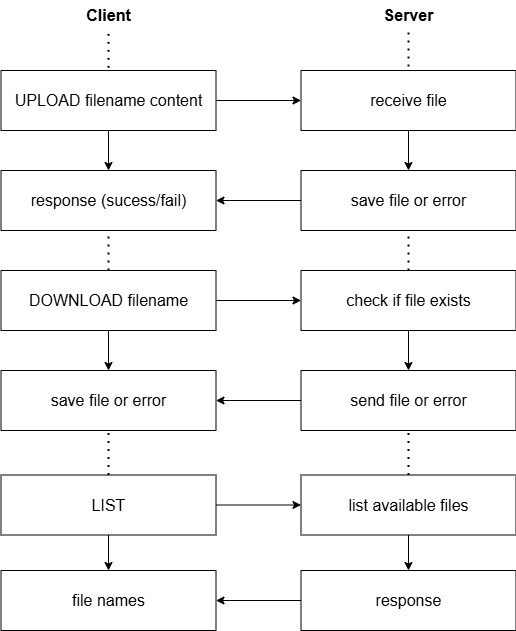
\includegraphics[width=\textwidth]{protocol_design.png} % Replace with your diagram
    \caption{Protocol Design}
    \label{fig:protocol}
\end{figure}

\section*{System Organization}
The system consists of two main components:
\begin{itemize}
    \item \textbf{Server:} Listens for client connections and handles file operations.
    \item \textbf{Client:} Connects to the server to perform upload, download, and list operations.
\end{itemize}

\begin{figure}[h]
    \centering
    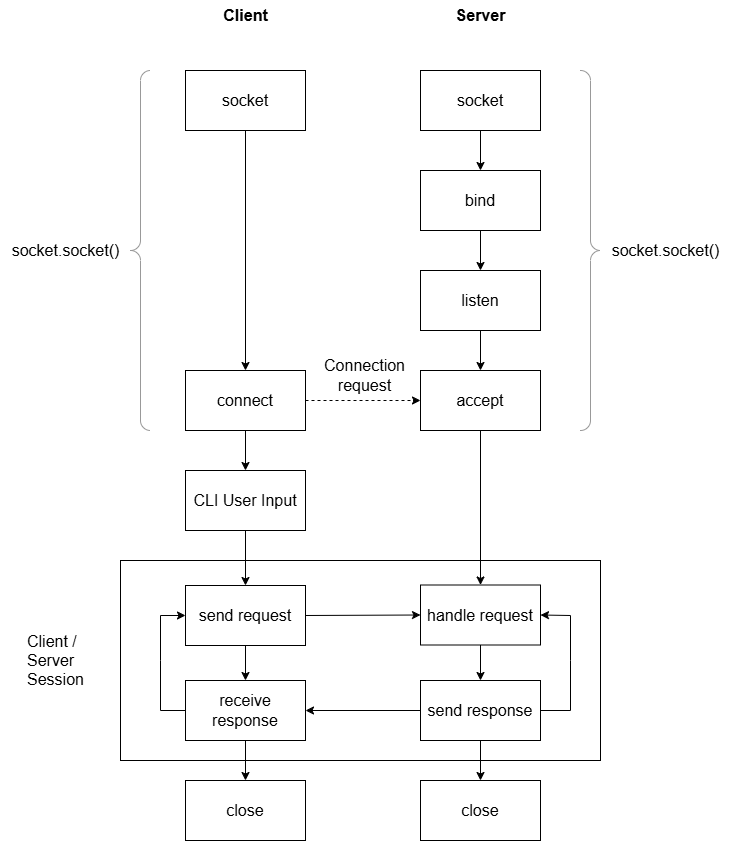
\includegraphics[width=\textwidth]{system_organization.png} % Replace with your diagram
    \caption{System Organization}
    \label{fig:system}
\end{figure}

\section*{Implementation}
\subsection*{File Transfer Logic}
The file transfer is implemented using Python's \texttt{socket} module. The server processes incoming requests and performs file I/O operations, while the client sends commands and processes responses.

\subsection*{Code Snippets}
\subsubsection*{Client Implementation}
\begin{lstlisting}[language=Python, caption=Client Implementation, label=lst:client, basicstyle=\ttfamily\footnotesize, keywordstyle=\color{blue}]
def send_request(request):
    try:
        s = socket.socket(socket.AF_INET, socket.SOCK_STREAM)
        s.connect((ip, port))
        s.sendall(request.encode())

        response = s.recv(1024).decode()
        s.close()
        return response
    except ConnectionRefusedError:
        return "Connection refused. Make sure the server is running."
    except socket.error as e:
        return f"Socket error: {e}"
    finally:
        s.close()


def upload():
    filename = input("Enter filename to upload: ").strip()

    if not os.path.exists(filename):
        return "File does not exist"

    with open(filename, "r") as file:
        content = file.read()

    request = f"UPLOAD {filename} {content}"
    response = send_request(request)

    return response


def download():
    filename = input("Enter filename to download: ").strip()
    request = f"DOWNLOAD {filename}"
    response = send_request(request)

    if "File not found" not in response:
        with open(filename, "wb") as f:
            f.write(response.encode())
        response = f"File {filename} downloaded successfully."

    return response


def list():
    request = "LIST"
    response = send_request(request)

    return response

\end{lstlisting}

\subsubsection*{Server Implementation}
\begin{lstlisting}[language=Python, caption=Server Implementation, label=lst:server, basicstyle=\ttfamily\footnotesize, keywordstyle=\color{blue}]
def handle_request(request, conn):
    parts = request.split(" ", 2)
    operation = parts[0]

    if operation == "UPLOAD":
        filename = parts[1]
        content = parts[2]

        with open(filename, "w") as f:
            f.write(content)
        return "File uploaded successfully"

    elif operation == "DOWNLOAD":
        filename = parts[1]

        if os.path.exists(filename):
            with open(filename, "rb") as f:
                content = f.read()
            conn.sendall(content)
            return ""
        else:
            return "File not found"

    elif operation == "LIST":
        files = os.listdir(".")
        return " ".join(files)

    else:
        return "Invalid operation"


def start_server(port):
    try:
        s = socket.socket(socket.AF_INET, socket.SOCK_STREAM)
        s.bind(("0.0.0.0", port))  # Bind to all available interfaces
        s.listen(5)
        print(f"Server started and listening on port {port}")

        while True:
            conn, addr = s.accept()
            try:
                request = conn.recv(1024).decode()
                response = handle_request(request, conn)
                if response:
                    conn.sendall(response.encode())
                print(f"Request: {request} | Response: {response}")
            except Exception as e:
                conn.sendall(f"Error processing request: {e}".encode("utf-8"))
                print(f"Request: {request} | Error processing request: {e}")
            finally:
                conn.close()
    except socket.error as e:
        print(f"Socket error: {e}")
    except Exception as e:
        print(f"Server error: {e}")
    finally:
        s.close()
\end{lstlisting}

\section*{Summary}
This system demonstrates a basic file transfer protocol over TCP/IP using Python sockets. The implementation supports essential file operations and provides a foundation for more advanced features such as authentication, encryption, and robust error handling.

\end{document}
